\section{Benutzertests}

Wie im Dokument ``Ergonomic Criteria for the Evaluation of Human-Computer Interfaces'' spezifiziert, stellt eine kriterienbasierte Bewertungsmethode lediglich einen analytischen Ansatz dar.
Als solche sind die Kriterien nicht dazu gedacht, andere Bewertungsmethoden zu ersetzen.
Daher sind Benutzertests weiterhin notwendig, um die Leistung und Nutzbarkeit einer Schnittstelle zu gewährleisten.
Aus diesem Grund wurden Benutzertests entwickelt, um allgemeine Usability-Probleme zu identifizieren und potenziell Probleme zu erkennen, die nicht von den Kriterien abgedeckt werden.

Das Ziel dieses Tests ist es, die Effektivität, Effizienz und Zufriedenheit mit der Silvanet-Webanwendung mithilfe von echten Nutzern zu quantifizieren.
Zunächst muss jedoch definiert werden, was getestet werden soll und vor allem, wie getestet werden soll.

\subsection{Festlegung der Testabdeckung}

Um relevante und schnelle Tests für die Benutzer durchführen zu können, mussten wir festlegen, auf welche Bereiche der Benutzeroberfläche sich die Tests konzentrieren sollten.
Es erschien uns sinnvoll, eine Gruppenaktivität mit dem Cloud-Team durchzuführen, um Ideen zu sammeln und die am meisten erwähnten auszuwählen.
Um die Brainstorming-Sitzung zu strukturieren und zu vermeiden, dass man sich zu sehr verzettelt, basiert die Aktivität auf der Ideationstechnik namens \textit{Lotus Blossoms}, die es ermöglicht, eine Idee nach der anderen gründlich zu erforschen.
Diese von S. Tatsuno 1990\cite{lotusBlossoms} entwickelte Methode der Ideenfindung lässt sich leicht durch das folgende Flussdiagramm schematisieren.

\begin{figure}[H]
  \centering
  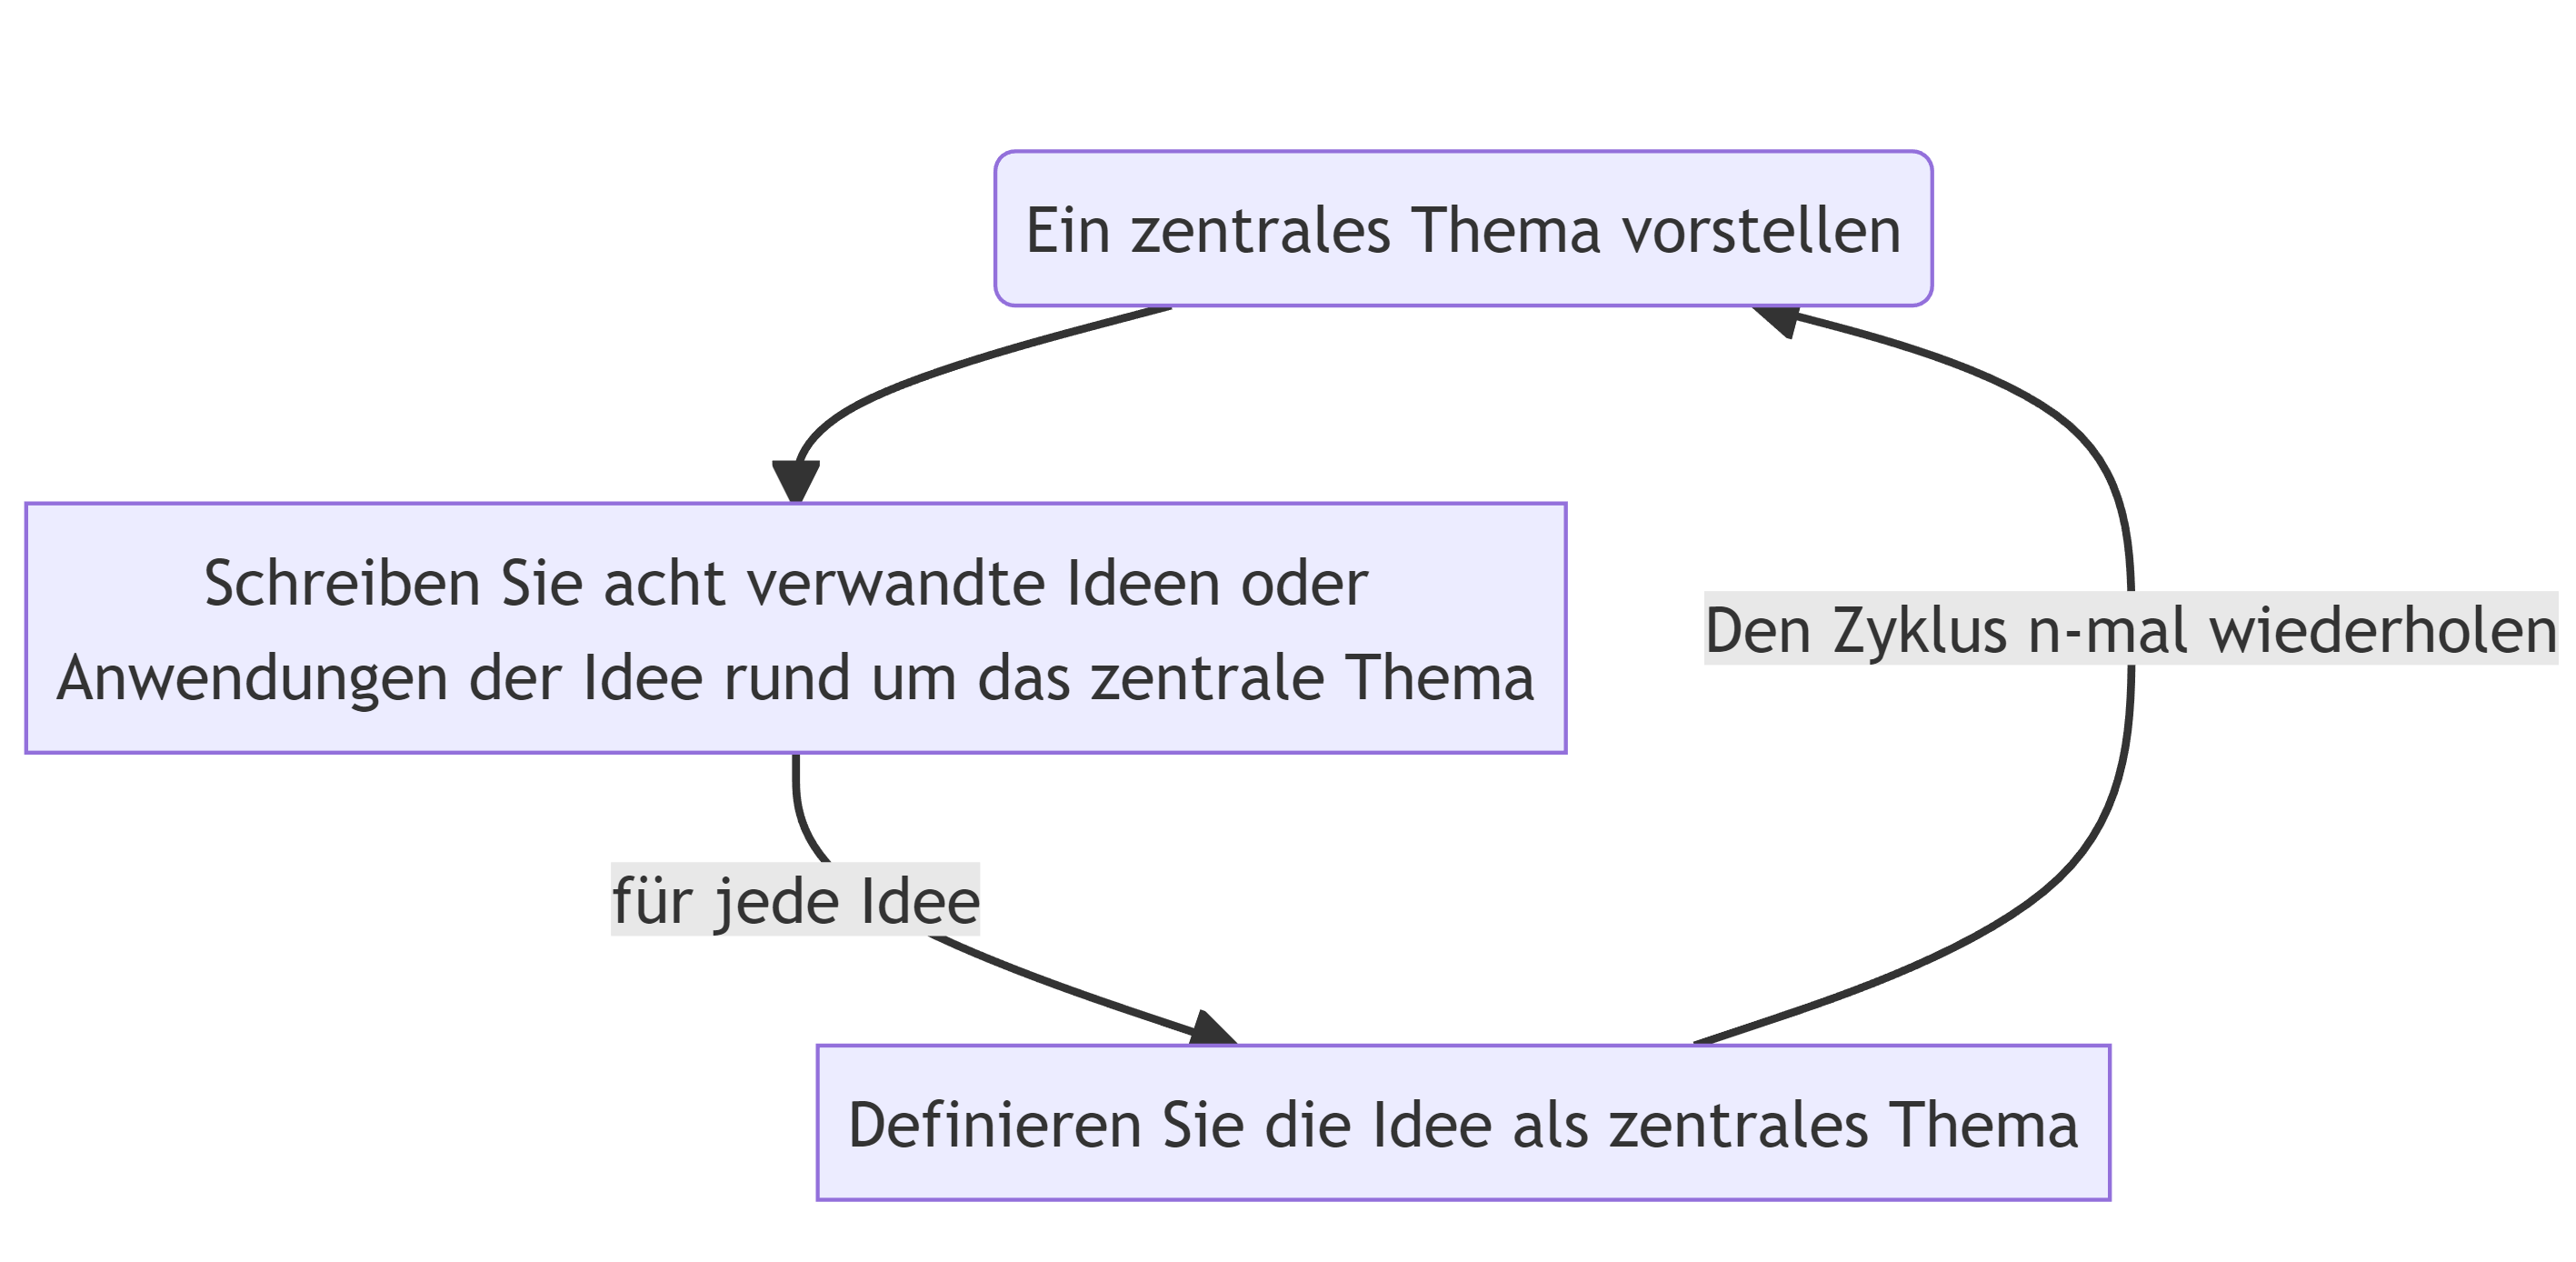
\includegraphics[width=\textwidth]{lotus_blossoms_flowdiagram}
  \caption{Darstellung eines Ideationszyklus mit der Lotus-Blossom-Methode}
  \label{fig:lotus_blossoms_flowdiagram}
\end{figure}

In diesem Fall sollte eine Iteration von zwei Zyklen ausreichen, um die wesentlichen Funktionen der Anwendung zu definieren.
Die erste zentrale Frage wurde im Vorfeld mit der Frage ``Was sind die Ziele des Gesprächs mit dem Kunden über die Anwendung?'' festgelegt.
Aus dieser Frage ergaben sich 6 verschiedene andere Themen:

\begin{itemize}
  \item Welche Informationen über die Geräte sind von Interesse?
  \item Ist die Planung eines \textit{Site} funktionsfähig und die Schnittstelle funktionstüchtig?
  \item Welche kundenorientierten Funktionen sollten den Nutzern zur Verfügung gestellt werden?
  \item Welche Art von Informationen würden Sie im Falle eines Feueralarms interessieren?
  \item Welche Art von Informationen möchten Sie auf dem Dashboard sehen?
  \item Funktioniert die Kartendarstellung gut?
\end{itemize}

\begin{figure}[H]
  \centering
  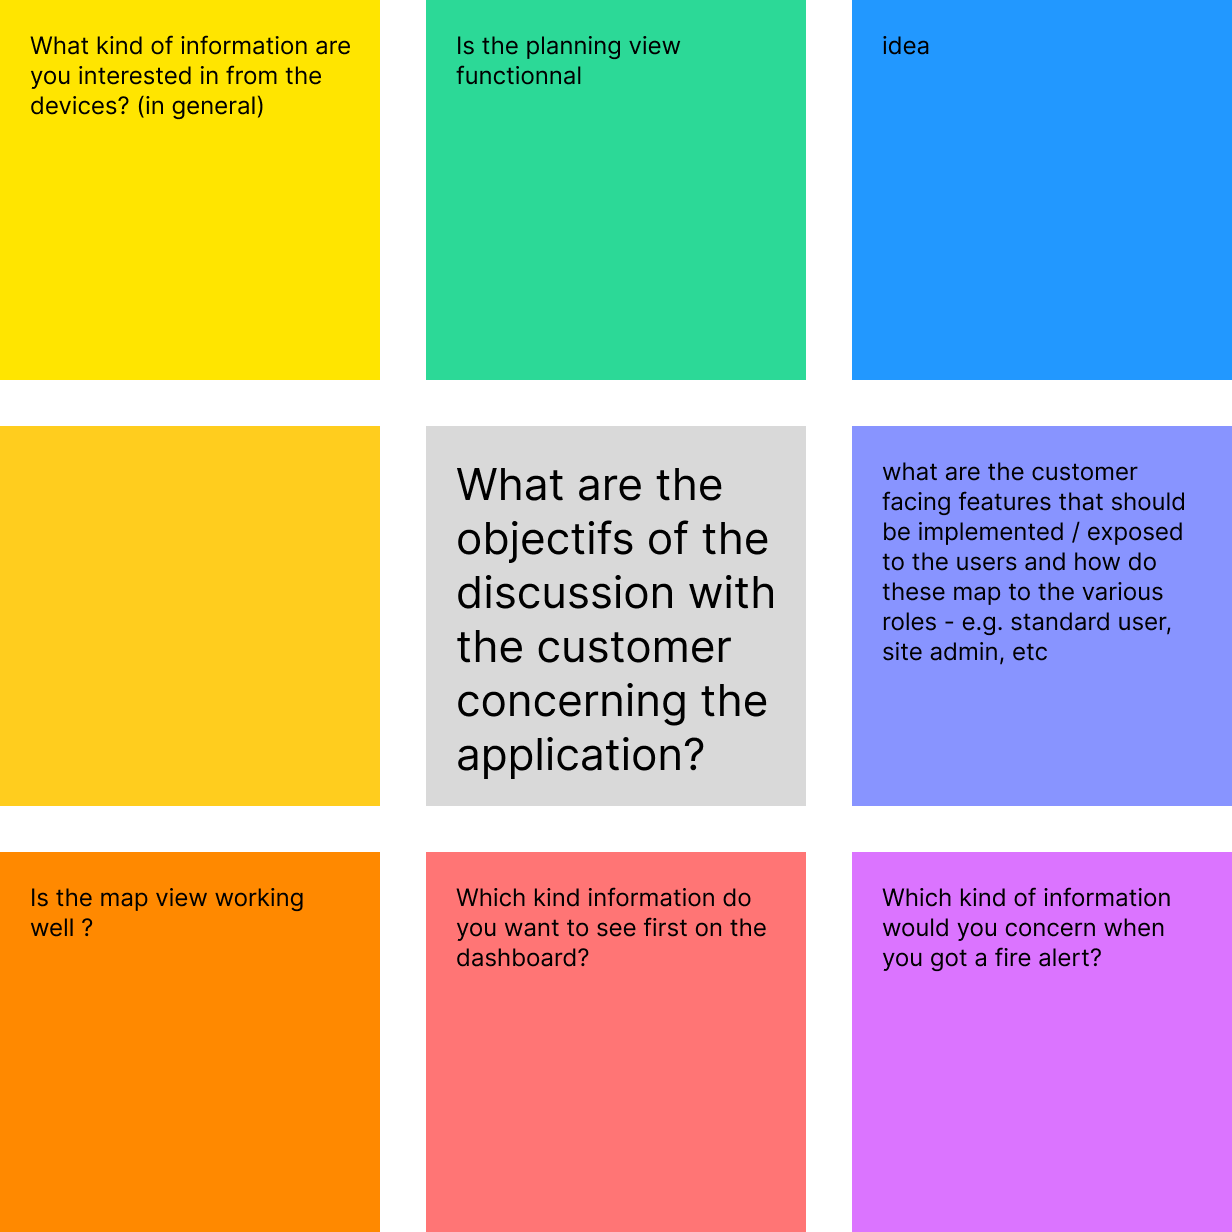
\includegraphics[width=10cm]{dryad_lotus_blossom_cycle_1}
  \caption{Durchführung des ersten Ideationszyklus durch das Cloud-Team von Dryad mit der Lotus-Blossom-Methode}
  \label{fig:dryad_lotus_blossom_cycle_1}
\end{figure}

In der zweiten Iteration wurden mehr Fragen zu den Funktionen der Benutzeroberfläche gestellt, die die genannten Themen beantworten oder näher erläutern können.

\begin{figure}[H]
  \centering
  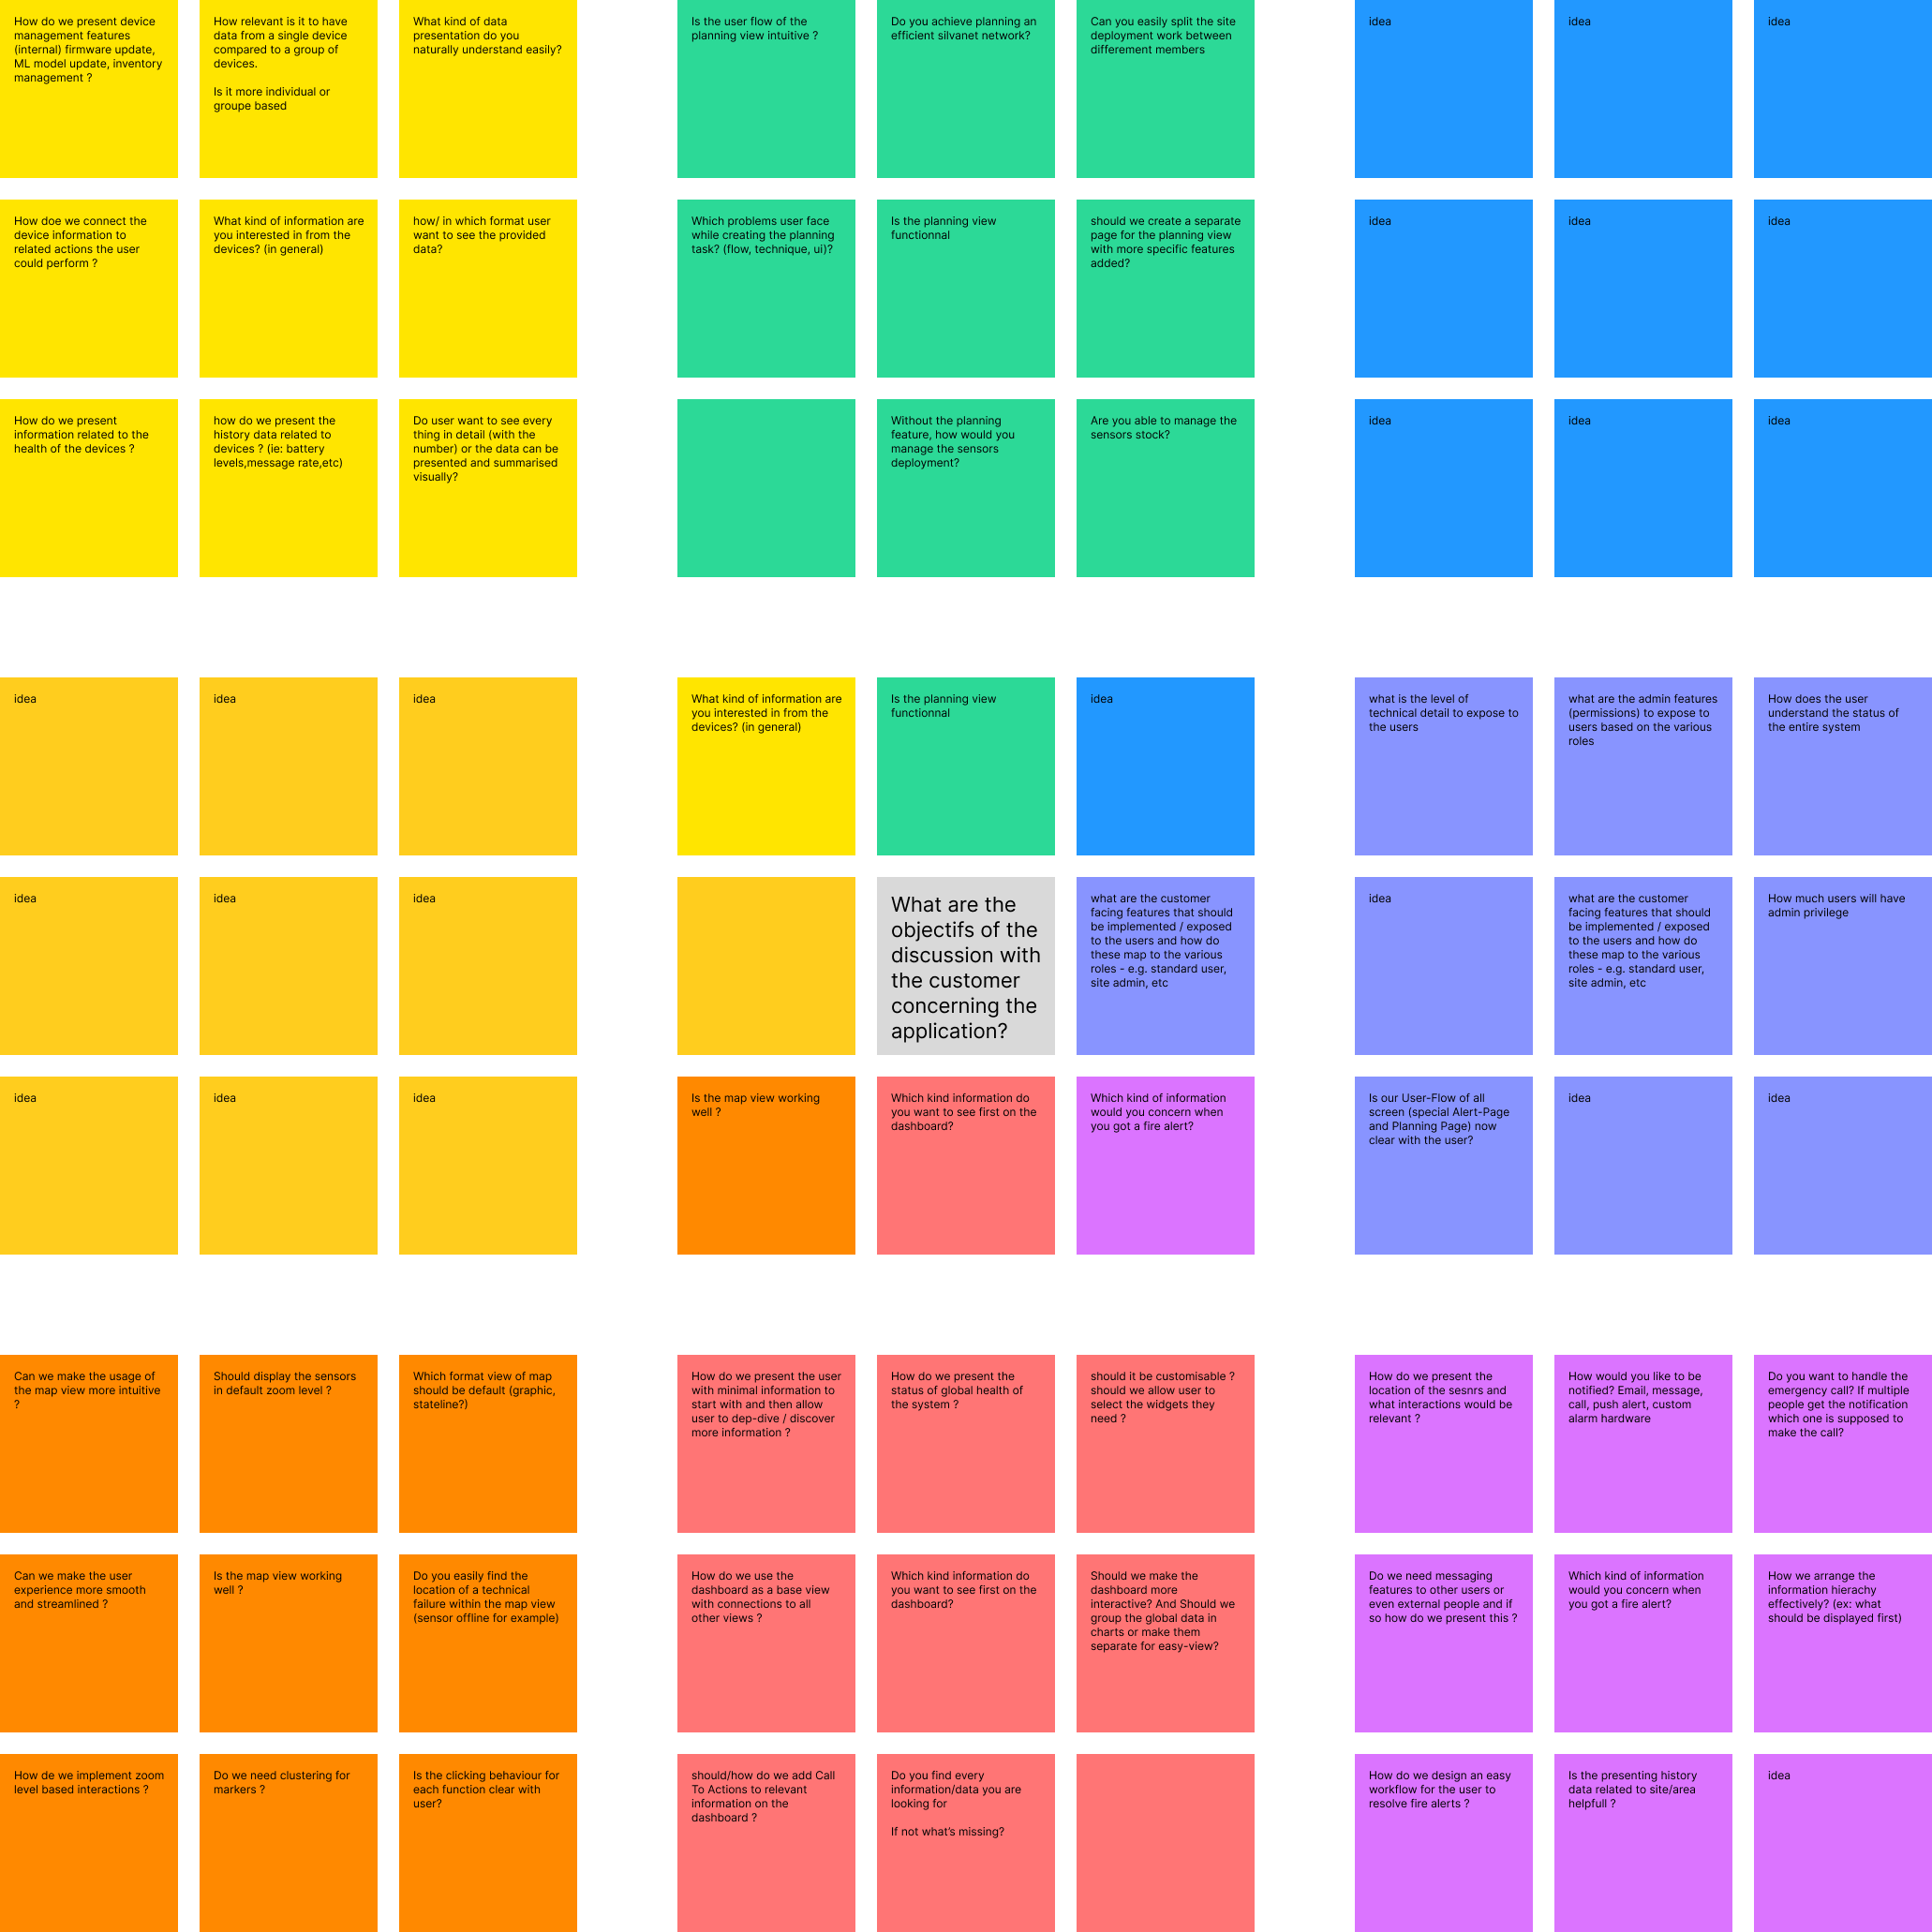
\includegraphics[width=\textwidth]{dryad_lotus_blossom_cycle_2}
  \caption{Durchführung des zweiten Ideationszyklus durch das Cloud-Team von Dryad mit der Lotus-Blossom-Methode}
  \label{fig:dryad_lotus_blossom_cycle_2}
\end{figure}

Die Einzelheiten zu den verschiedenen Blütenblättern der Lotus Blossom des zweiten Zyklus können im Anhang \ref{appendix:lotus_blossom} eingesehen werden.\\

Diese Aktivität ermöglichte es, die Usability-Tests schließlich auf die folgenden Features zu konzentrieren:

\begin{itemize}
  \item \textbf{Planung der Sensoren eines \textit{Site} \ac{UX}}: Die Anwendung bietet dem Nutzer eine Seite, auf der er auf einer interaktiven Karte die neuen Sensoren an einem \textit{Site} so positionieren kann, dass die Erfassungsabdeckung der Sensoren optimiert wird. Dies führt den Nutzer dann durch den Wald zu den Koordinaten, an denen er einen Sensor hoch oben an einem Baum befestigen muss.
  \item \textbf{Relevanz der Information in Alarmsituationen}: Wenn ein Feuer vom System erkannt wird, hat der Benutzer Zugang zu einer Alarmseite, die die Situation mithilfe von Daten und einer interaktiven Karte detailliert darstellt. Es sind auch schnelle Aktionen möglich, wie z.B. die Kontaktaufnahme mit den örtlichen Behörden. Dies betrifft auch Informationen, die per E-Mail an den Nutzer gesendet werden, um ihn über den Alarm zu benachrichtigen.
  \item \textbf{Usability der interaktiven Karte}: Die Anwendung bietet eine Seite, die nur aus einer interaktiven Karte besteht, auf der Sie die verschiedenen \textit{Sites} und Sensoren anhand ihrer geografischen Lage einsehen können.
  \item \textbf{Relevanz von Sensordaten}: In der Anwendung werden die Sensordaten auf unterschiedliche Weise dargestellt. Es wäre interessant, die Strategie zu definieren, die verwendet wird, um diese Daten für den Benutzer relevant zu präsentieren.
\end{itemize}

\subsection{Methoden für Usability-Tests}

Nachdem der Fokus der Usability-Tests festgelegt wurde, ist es nun an der Zeit festzulegen, wie die Tests durchgeführt werden sollen, um in kurzer Zeit möglichst viel relevantes Feedback zu erhalten.
In der von \citeauthor{usability} durchgeführten und in \citetitle{usability} erläuterten Forschung gibt es zwei Techniken, die zusammen eine gute Abdeckung der Usability einer Schnittstelle ermöglichen.

\subsubsection{Qualitative Bewertung}

Die erste besteht in der Entdeckung und Lösung von Usability-Problemen.
Studien zur Problementdeckung zeichnen sich dadurch aus, dass sie sehr informell sind.
Der Schwerpunkt liegt nicht auf der genauen Messung der Leistung oder der Haltung der Teilnehmer, sondern auf einer starken Interaktion zwischen Beobachtern und Teilnehmern.
Die Durchführung dieser Tests ist einfach, da sie auf spezifischen Zielen zur Entdeckung eines Problems basieren, wie z. B. ``Identifizieren Sie einen Sensor an der Schnittstelle, der das Vorhandensein von Rauch detektiert''.
Diese informellen Tests, die mehrmals mit vielen verschiedenen Nutzern wiederholt werden, ermöglichen eine umfassendere Problemerkennung, insbesondere solche, an die die Tester nicht gedacht hätten.
Aus diesem Grund wird eine Reihe solcher Tests für freiwillige Nutzer angeboten.

\subsubsection{Quantitative Bewertung}

Die zweite Methode wird auf einer quantitativen Bewertung der Schnittstelle basieren, die es ermöglicht, eine Usability-Skala zu erhalten, mit der man einfach die Entwicklung der Schnittstelle im Vergleich zur vorherigen Version vergleichen kann, indem man einfach die Bewertungen vergleicht.
Eine weit verbreitete Technik der quantitativen Bewertung basiert auf dem Maß der percuted utilisability, kurz \ac{SUS} genannt\cite{usability}.
\ac{SUS} ist ein standardisierter Fragebogen, der 10 Fünf-Punkte-Items mit abwechselnd positiver und negativer Tonalität enthält. Die Inhalte der Items sind wie folgt:

\begin{enumerate}
  \item I think that I would like to use this system frequently.
  \item I found the system unnecessarily complex.
  \item I thought the system was easy to use.
  \item I think that I would need the support of a technical person to be able to use this system.
  \item I found the various functions in this system were well integrated.
  \item I thought there was too much inconsistency in this system.
  \item I would imagine that most people would learn to use this system very quickly.
  \item I found the system very awkward to use.
  \item I felt very confident using the system.
  \item I needed to learn a lot of things before I could get going with this system.
\end{enumerate}

Für jeden Punkt muss der Nutzer dann eine Bewertung zwischen \textbf{1} und \textbf{5} abgeben, wobei \textbf{1} für \textit{Stimmt überhaupt nicht zu} und \textbf{5} für \textit{Stimme voll und ganz zu} steht. Wenn der Nutzer kein Urteil hat, kann er die Note \textbf{3} geben, die neutral ist.
Wenn Sie fertig sind, können Sie die Gesamtpunktzahl anhand der Punktzahl jedes Items berechnen, die auf eine Skala zwischen 0 und 4 gebracht wird.
Bei positiv formulierten Items (1, 3, 5, 7 und 9) ist der Beitrag zur Punktzahl die Position auf der Skala minus 1.
Bei negativ formulierten Items (2, 4, 6, 8 und 10) ist der Beitrag zur Punktzahl gleich 5 minus der Position auf der Skala.
Um die Gesamtpunktzahl des SUS zu erhalten, muss die Summe der Punktzahlen der einzelnen Items mit 2,5 multipliziert werden.
So reichen die SUS-Scores von 0 bis 100 in Schritten von 2,5 Punkten.\\

Schließlich kann die Punktzahl einer Schnittstelle mithilfe der folgenden Skala adjektiviert werden:

\begin{itemize}
  \item (score <= 25): Unvorstellbar schlecht
  \item (25 < score <= 51,7): Schlecht
  \item (51,7 < score <= 71,7): Fair
  \item (71,7 < score <= 80,7): Gut
  \item (80,7 < score <= 84,1): Ausgezeichnet
  \item (84,1 < score): Das Beste, was man sich vorstellen kann
\end{itemize}

\begin{figure}[H]
  \centering
  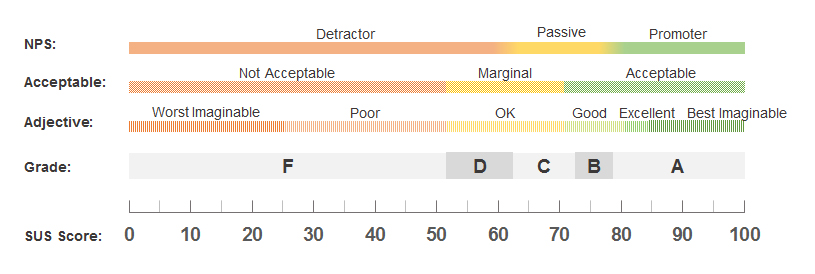
\includegraphics[width=\textwidth]{sus_scala}
  \caption{Noten, Adjektive, Akzeptanz und NPS-Kategorien in Verbindung mit den SUS-Rohwerten\cite{sus_scala}}
  \label{fig:sus_scala}
\end{figure}

\subsubsection{Bewertung durch Vergleich}

Wenn ein Nutzerproblem gut bekannt ist und bereits eine oder mehrere Verbesserungsideen vorgeschlagen wurden, ist es sinnvoll, die relevanteste mithilfe eines Vergleichstests zu bewerten.
Die Idee dahinter ist sehr einfach: Dem Benutzer wird eine Aktion gegeben, die er auf zwei Schnittstellen ausführen muss. Am Ende des Tests wählt der Benutzer aus, welche Schnittstelle er bevorzugt hat.
Wenn die Schnittstellen nicht entwickelt werden, reichen einfache Screenshots zum Vergleich aus.
Dieses Vergleichsverfahren hat einen Namen, der häufiger verwendet wird: \textit{A/B-Testing}.

\subsubsection{Techniken der Tester-Nutzer-Interaktion}

Da ein Teil der Tests informell ist, ist es notwendig, Testmethoden zu definieren, um zu verhindern, dass die Diskussion zu sehr abschweift, und gleichzeitig so viel Feedback wie möglich zu erhalten.
Eine einfach umzusetzende Idee und das Erhalten eines mündlichen Berichts vom Nutzer mithilfe der \ac{TA}-Technik (\textit{Lautes Denken} auf Deutsch).
Dazu muss der Tester nur angeben, dass er mit dem Benutzer darüber sprechen möchte, was er tut, während er es tut.
Wenn die Teilnehmer aufhören zu sprechen, was häufig vorkommt, wenn sie mit einer Aufgabe sehr beschäftigt sind, werden sie aufgefordert, das Sprechen wieder aufzunehmen.\\

Auch aus Gründen des Mangels an potenziellen Nutzern in der Nähe der Büros des Unternehmens werden die Usability-Tests synchron aus der Ferne durchgeführt.
Dies hat den großen Vorteil, dass wir Zugang zu internationalen Teilnehmern haben und ihnen die Möglichkeit bieten, in einer vertrauten Umgebung zu arbeiten, die eine mittelmäßig verzerrte Testdurchführung ermöglicht.
Auch wenn dieser Ansatz weniger interaktiv zu sein scheint als in der Nutzerpräsenz, haben Tests gezeigt, dass die Ergebnisse mit den Ergebnissen vergleichbar sind, die mit traditionelleren Tests erzielt werden\cite{remoteUsabilityEvaluation}.

\subsection{Aufbau von Usability-Tests}

Nachdem wir festgelegt haben, was wir testen und wie wir es testen, ist es an der Zeit, unsere Tests und die benötigten Medien zu definieren.
Zehn Hauptthemen ergeben sich aus der Definition des Testabdeckung:

\begin{enumerate}
  \item \textbf{Gerätefehlererkennung}: Fähigkeit des Nutzers, mithilfe der interaktiven Karte Streitigkeiten an den Sensoren eines \textit{Site} zu erkennen.
  \item \textbf{Offline-Sensorerkennung}: Fähigkeit des Nutzers, einen Sensor zu erkennen, der offline auf der interaktiven Karte angezeigt wird.
  \item \textbf{Erschwinglichkeit des Sicherheitsdesigns}: Fähigkeit der Schnittstelle der interaktiven Karte, dem Nutzer zu vermitteln, dass ein \textit{Site} sicher ist oder nicht.
  \item \textbf{Karte überlagern}: Welcher Kartentyp zwischen Satellitenansicht und Planansicht am besten geeignet ist, hängt von der Lage zwischen Wald und Stadtgebiet ab.
  \item \textbf{Erstellung von Einsatzpaketen}: Fähigkeit des Nutzers, Sensoren zu planen, die an einem \textit{Site} installiert werden sollen.
  \item \textbf{Ausgabe des Einsatzpakets}: Fähigkeit des Benutzers, ein geplantes Sensorpaket für einen \textit{Site} zu bearbeiten.
  \item \textbf{Ablauf des Feueralarms}: Fähigkeit des Benutzers, bei einem Waldbrand schnell einen \textit{Site} zu identifizieren.
  \item \textbf{Notruf}: Fähigkeit des Nutzers, bei einer Warnung die zuständigen Behörden zu kontaktieren.
  \item \textbf{Teilen von Feueralarm}: Fähigkeit des Nutzers, den Alarmstatus teilen zu wollen und zu können.
  \item \textbf{Reaktion auf Feueralarm-E-Mails}: Reaktion und Verhalten des Nutzers auf eine E-Mail mit Waldbrandalarm.
\end{enumerate}

Diese Themen werden mit dem Nutzer in der gleichen Reihenfolge besprochen.
Die beiden Themen \textbf{Karte überlagern} und \textbf{Reaktion auf Feueralarm-E-Mails} werden mithilfe eines A/B-Tests quantifizierend gemessen.
Die anderen Themen werden informelle Usability-Tests sein, die die \ac{TA}-Methode verwenden und auf einfachen Aufgaben basieren, die auf der Silvanet-Schnittstelle direkt ausgeführt werden müssen.
Die Aufgabenstellung für die verschiedenen Aufgaben lautet wie folgt:

\begin{table}[H]
  \begin{tabular}{p{0.3\linewidth} |p{0.7\linewidth}}
    Thema                                             & Aufgabenstellung                                                                                                                                                                                                                                                                                                  \\ \hline\hline

    \textbf{Gerätefehlererkennung}                    & Derzeit gibt es ein Problem mit einigen Geräten auf einer der \textit{Site}. Lokalisieren Sie sie mit Hilfe der Kartenansicht und teilen Sie mir mit, wo das Problem liegt. Wenn Sie fertig sind, sagen Sie bitte "Ich bin fertig.".                                                                              \\\hline
    \textbf{Offline-Sensorerkennung}                  & Es gibt einen \textit{Site} namens "Eberswalde B", der einen Offline-Sensor hat. Nennen Sie mir in der Standortübersicht den Namen/die Kennung des Geräts. Wenn Sie fertig sind, sagen Sie bitte "Ich bin fertig".                                                                                                \\\hline
    \textbf{Erschwinglichkeit des Sicherheitsdesigns} & Wählen Sie in der Kartenansicht einen \textit{Site} Ihrer Wahl und sagen Sie mir, ob er sicher ist oder nicht und warum. Wenn Sie fertig sind, sagen Sie bitte "Ich bin fertig".                                                                                                                                  \\\hline
    \textbf{Erstellung von Einsatzpaketen}            & Erstellen Sie ausgehend von der \textit{Site}ansicht ein neues Einsatzpaket für den Standort "Eberswalde Demo", das 1 \textit{Mesh-Gateway} und 2 Sensoren enthält. Platzieren Sie diese in gleichem Abstand auf der Karte, um das Paket fertigzustellen. Wenn Sie fertig sind, sagen Sie bitte "Ich bin fertig". \\\hline
    \textbf{Ausgabe des Einsatzpakets}                & Bearbeiten Sie den Namen des Pakets, das Sie gerade erstellt haben. Danach entfernen Sie es. Wenn Sie fertig sind, sagen Sie bitte "Ich bin fertig".                                                                                                                                                              \\\hline
    \textbf{Ablauf des Feueralarms}                   & Es gibt einen Feueralarm in einem Ihrer \textit{Sites}. Sagen Sie laut, an welchem \textit{Site} und wo das Feuer ungefähr ausgebrochen ist. Wenn Sie fertig sind, sagen Sie bitte "Ich bin fertig".                                                                                                              \\\hline
    \textbf{Notruf}                                   & Versuchen Sie, in der Brandmeldezentrale den Notdienst anzurufen. Sprechen Sie die Informationen, die Sie wahrscheinlich sagen werden, laut aus. Wenn Sie fertig sind, sagen Sie bitte "Ich bin fertig".                                                                                                          \\\hline
    \textbf{Teilen von Feueralarm}                    & Es brennt gerade und Sie wollen es mit einem Ihrer Mitarbeiter teilen. Was werden Sie tun? Wenn Sie fertig sind, sagen Sie bitte "Ich bin fertig".
  \end{tabular}
  \caption{Aktionen, die der Nutzer im Rahmen von Usability-Tests durchführen muss}
\end{table}

Im Anschluss an jede vom Nutzer durchgeführte Aktion sollte ihm ein \ac{SUS}-Fragebogen angeboten werden, um die empfundene Erfahrung zu quantifizieren.

\subsection{Ablauf der Usability-Tests}

Die Benutzertests werden im Remote-Modus durchgeführt, bei dem der Bildschirm des Benutzers geteilt wird, um seine Bewegung zu verfolgen.
Das Online-Videoanruftool \href{https://meet.google.com/}{Google Meet}\footnote{https://meet.google.com/} wird aus folgenden Gründen dafür verwendet:

\begin{enumerate}
  \item Out-of-the-Box-Webanwendung, die keine besondere Installation erfordert
  \item Verfügbare Dienste in den Regionen der Welt, auf die sich die Suche bezieht
  \item Kostenlose Lösung
\end{enumerate}

Die verschiedenen Anleitungen zur Durchführung von Usability-Tests und das dazugehörige \ac{SUS}-Formular werden dem Nutzer in Form eines Online-Fragebogens präsentiert, der mit dem Tool \href{https://www.google.com/forms/about/}{Google Form}\footnote{https://www.google.com/forms/about/}  erstellt wurde.
Die A/B-Tests werden dem Nutzer auch in der Google Form präsentiert.

\begin{figure}[H]
  \centering
  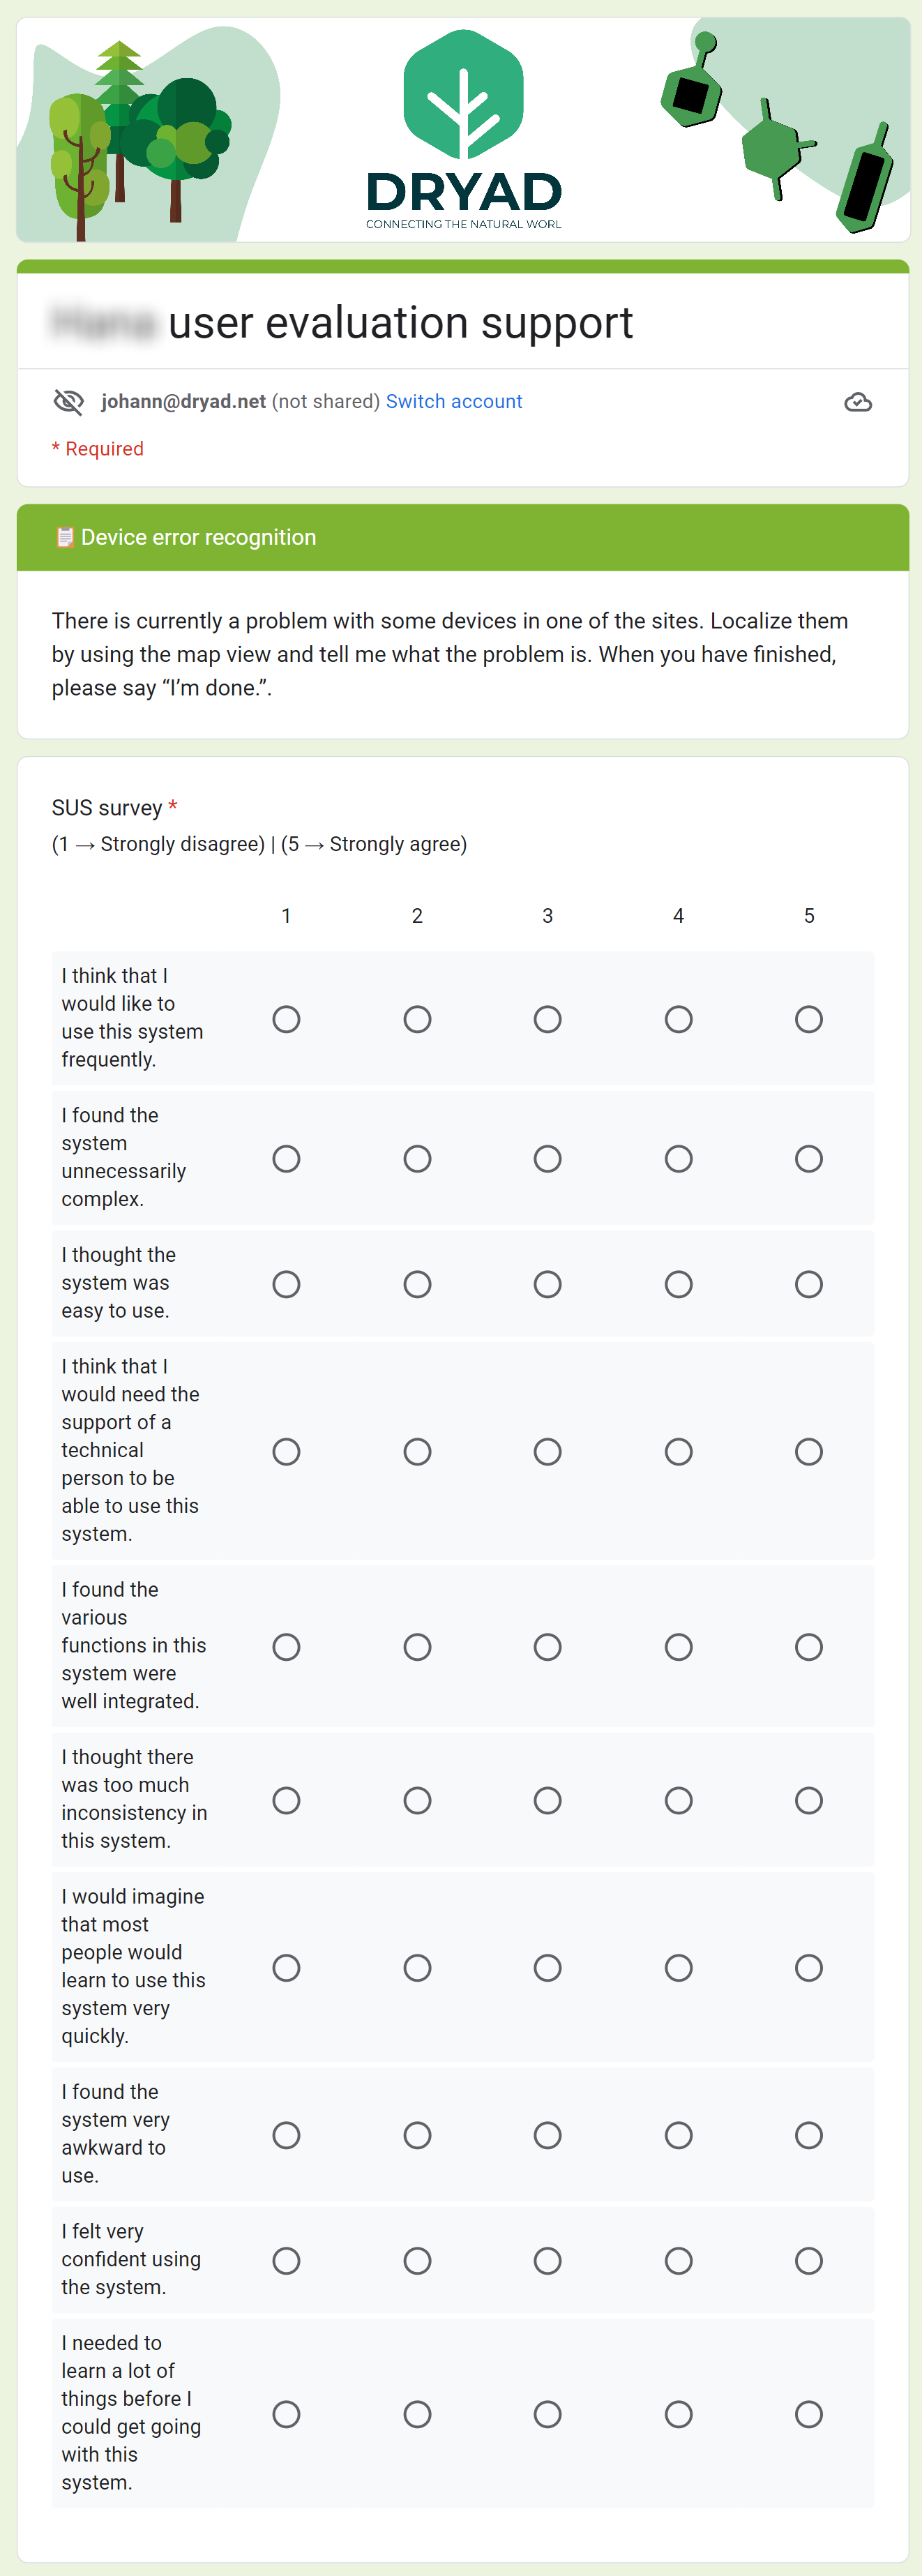
\includegraphics[width=8cm]{survey_question}
  \caption{Beispiel einer Frage aus dem Formular für die Usability-Forschung, das dem Benutzer vorgelegt wird}
  \label{fig:survey_question}
\end{figure}

\begin{figure}[H]
  \centering
  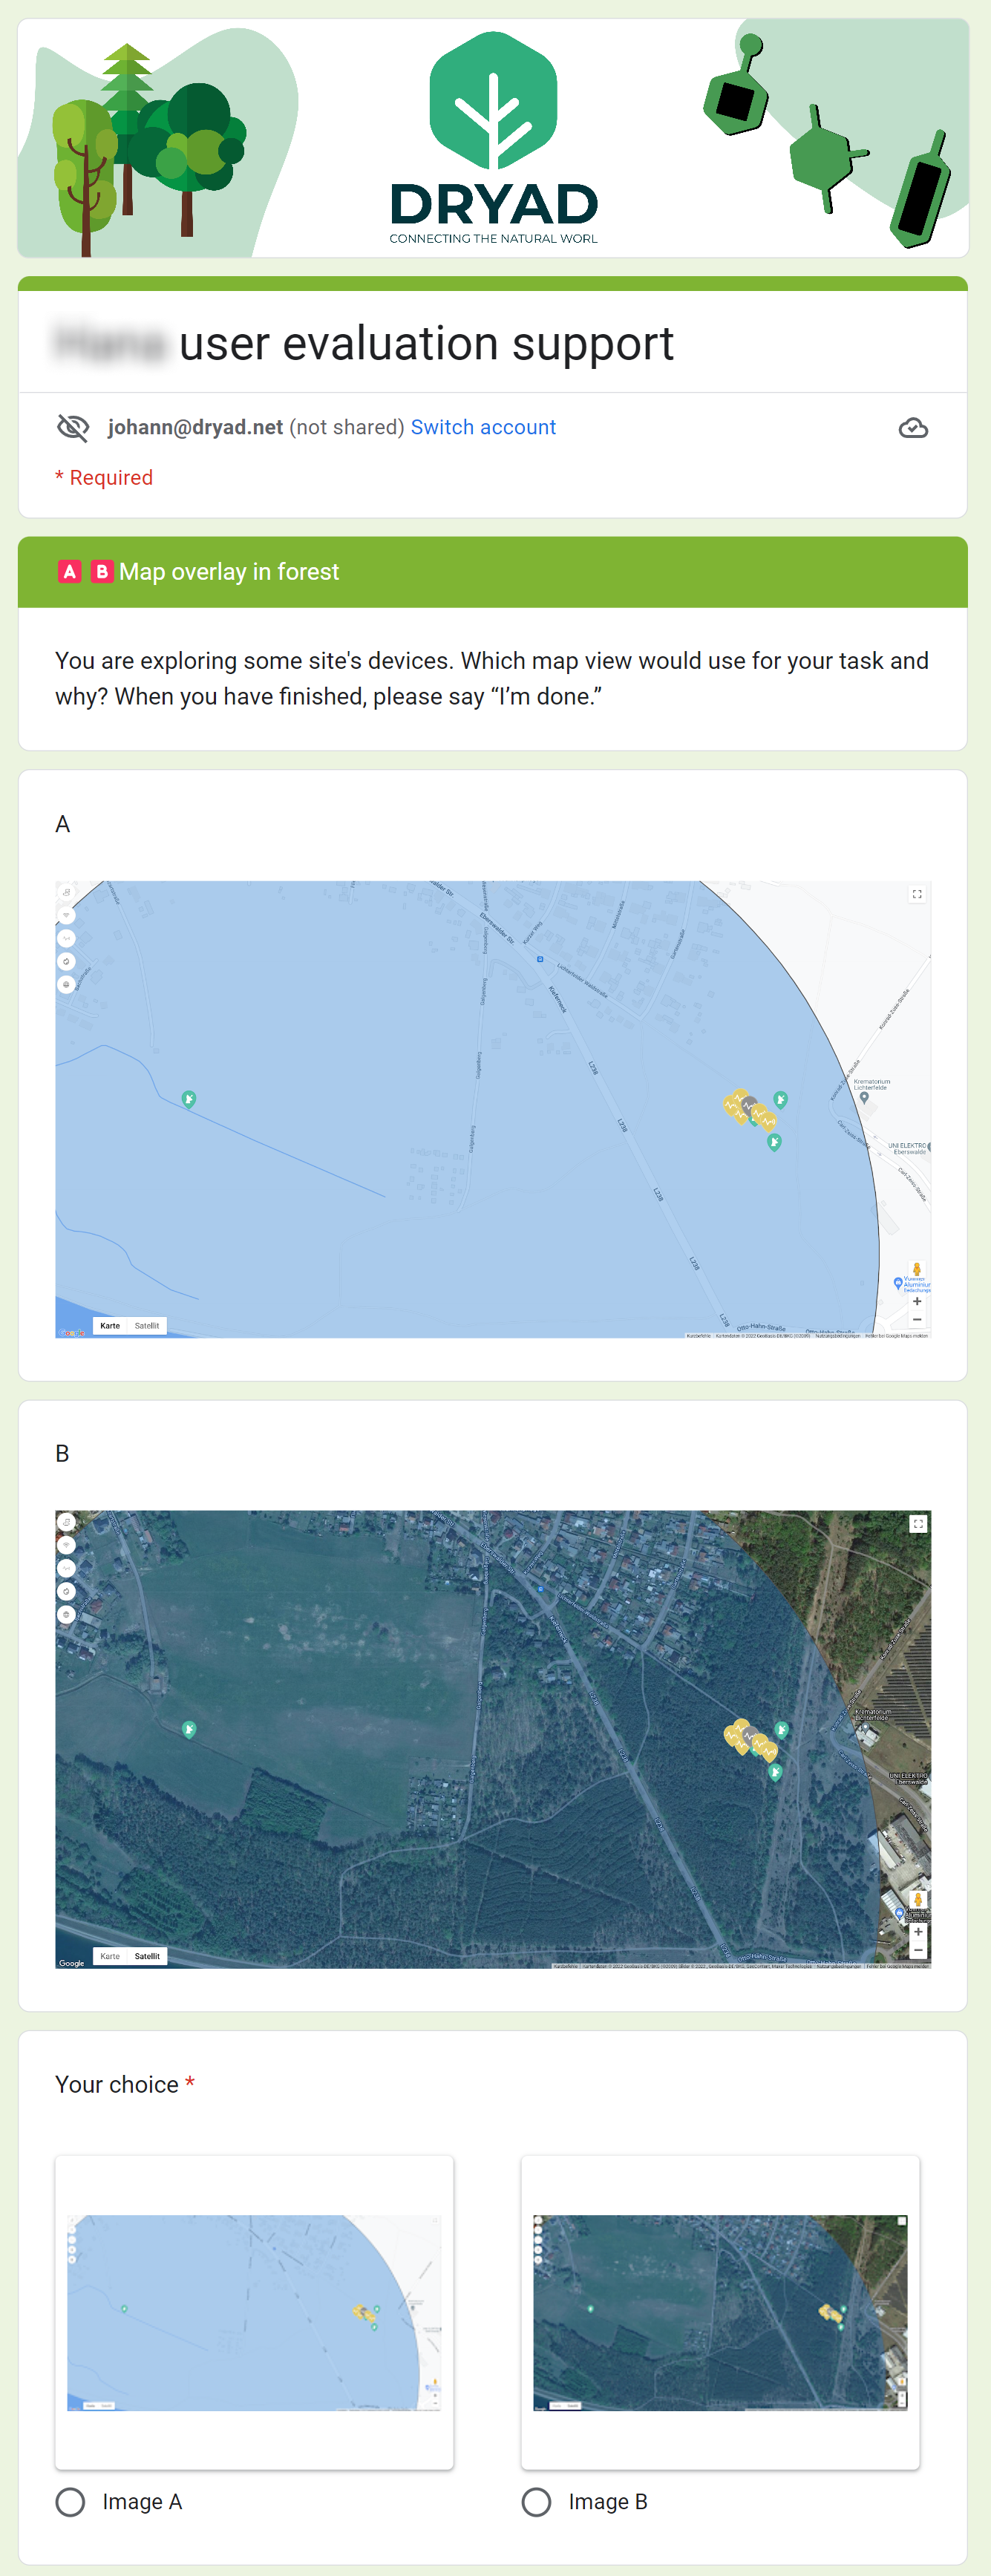
\includegraphics[width=8cm]{survey_ab_testing}
  \caption{Beispiel eines A/B-Vergleichs des Formulars für die Untersuchung der Usability, die dem Benutzer präsentiert wird}
  \label{fig:survey_ab_testing}
\end{figure}

Der Nutzer wird gefragt, ob er die Frage und die Aufgabe richtig verstanden hat, und muss dann die Aufgabe ausführen, während er die durchgeführten Aktionen mündlich erläutert.
Es werden Notizen über die Interaktion des Nutzers mit der Schnittstelle mittels Videoübertragung seines Bildschirms und über die mündlichen Erklärungen des Nutzers gemacht.
Wenn der Nutzer eine Frage oder Anmerkung hat, dann kann eine offene Diskussion gestartet werden, um ungeplantes Feedback zu erhalten.
Da die technische Leistung der Schnittstelle nicht quantifiziert wird, müssen die Benutzeraktionen für diese Tests nicht zeitlich festgelegt werden.\\

Nach einer Reihe von Pilottests, die mit drei Mitgliedern des Cloud-Teams von Dryad durchgeführt wurden, um Inkonsistenzen, Ungenauigkeiten oder Sprachfehler im Test und im Formular zu identifizieren, war es an der Zeit, den Usability-Test mit einem echten Benutzer durchzuführen.
Da Dryad noch ein junges Startup ist, ist die Anzahl der Kunden begrenzt und die, die bereit sind, sich eine Stunde Zeit zu nehmen, um an den Tests teilzunehmen, noch weniger.
Glücklicherweise war ein Kunde aus Südkorea bereit, bei dem Versuch, die Qualität des Produkts zu verbessern, zu helfen, indem er die Einladung zum Test annahm.

\subsection{Ergebnis der Benutzertests}

Letztendlich konnte nur ein Nutzer den Usability-Test vollständig bestehen.
Dies ist für ein relevantes und unvoreingenommenes Feedback wirklich zu vernachlässigen, aber leider war es nicht möglich, in der vorgegebenen Zeit mehr Kandidaten zu bekommen.
Die Testergebnisse bleiben dennoch sehr interessant.
Hier sind die \ac{SUS}-Bewertungen für die verschiedenen Themen, die für diesen Benutzer gesammelt wurden.

\begin{table}[H]
  \begin{tabular}{p{0.4\linewidth} |p{0.3\linewidth}|p{0.3\linewidth}}
    Thema                                             & \ac{SUS}-Bewertungen & Entsprechendes Adjektiv                 \\ \hline\hline

    \textbf{Gerätefehlererkennung}                    & 35                   & Schlecht                                \\\hline
    \textbf{Offline-Sensorerkennung}                  & 55                   & Schlecht                                \\\hline
    \textbf{Erschwinglichkeit des Sicherheitsdesigns} & 40                   & Schlecht                                \\\hline
    \textbf{Erstellung von Einsatzpaketen}            & 90                   & Das Beste, was man sich vorstellen kann \\\hline
    \textbf{Ausgabe des Einsatzpakets}                & 65                   & Fair                                    \\\hline
    \textbf{Ablauf des Feueralarms}                   & 95                   & Das Beste, was man sich vorstellen kann \\\hline
    \textbf{Notruf}                                   & 97.5                 & Das Beste, was man sich vorstellen kann \\\hline
    \textbf{Teilen von Feueralarm}                    & 67.5                 & Fair
  \end{tabular}
  \caption{Ergebnisse der SUS-Bewertungen nach Themenbereichen der Fragen.}
\end{table}

Diese Ergebnisse und das mündliche Feedback der Nutzer zeigen sehr deutlich, dass die Schnittstelle im Allgemeinen \textit{Fair} ist, außer bei den Punkten, die die interaktiven Karten betreffen, die alle als \textit{Schlecht} bezeichnet werden.
Diese Beobachtung ist für die Dryad-Teams keineswegs eine neue Erkenntnis, da sie die mangelnde Nutzbarkeit interaktiver Karten ebenso anerkennen.
Die Mehrheit der Probleme mit der interaktiven Karte wurden von den Nutzern wie folgt klar benannt.

\begin{enumerate}
  \item Unmöglichkeit, auf einer Gesamtansicht zu einer \textit{Site} zu navigieren
  \item Unverständnis, wenn beim Zoomen in eine \textit{Site} die Sensoren nicht angezeigt werden und nichts passiert.
  \item Die vielen verschiedenen Farben der Marker erschweren die Schlussfolgerung
  \item Unmöglichkeit, schnell zu erkennen, ob eine \textit{Site} ein Problem hat oder nicht
\end{enumerate}

A/B-Tests waren auch interessant, mündlich mit dem Nutzer direkt zu analysieren.
Die interaktiven Karten mit Satellitenansicht sind sogar in städtischen Gebieten besser geeignet als die mit Kartenansicht.
Der Nutzer erklärt, dass er häufiger die Satellitenansicht der Google Map-Anwendung nutzt, was die Erfahrung vertrauter macht.
Auch die Satellitenansicht ermöglicht es, die Bilder des Waldes sehr genau zu sehen.

Der andere A/B-Test war ebenfalls interessant. Ein Vorschlag für ein neues E-Mail-Design mit weniger Rohdaten und nur einem Link zur Warnseite der Anwendung wurde mit der aktuellen Version verglichen.
Der Nutzer fühlte sich sicherer, wenn er die E-Mail mit mehr Daten erhielt, da er so schneller und einfacher mit den Medien teilen konnte, die er gewöhnlich benutzt.

\begin{figure}[H]
  \centering
  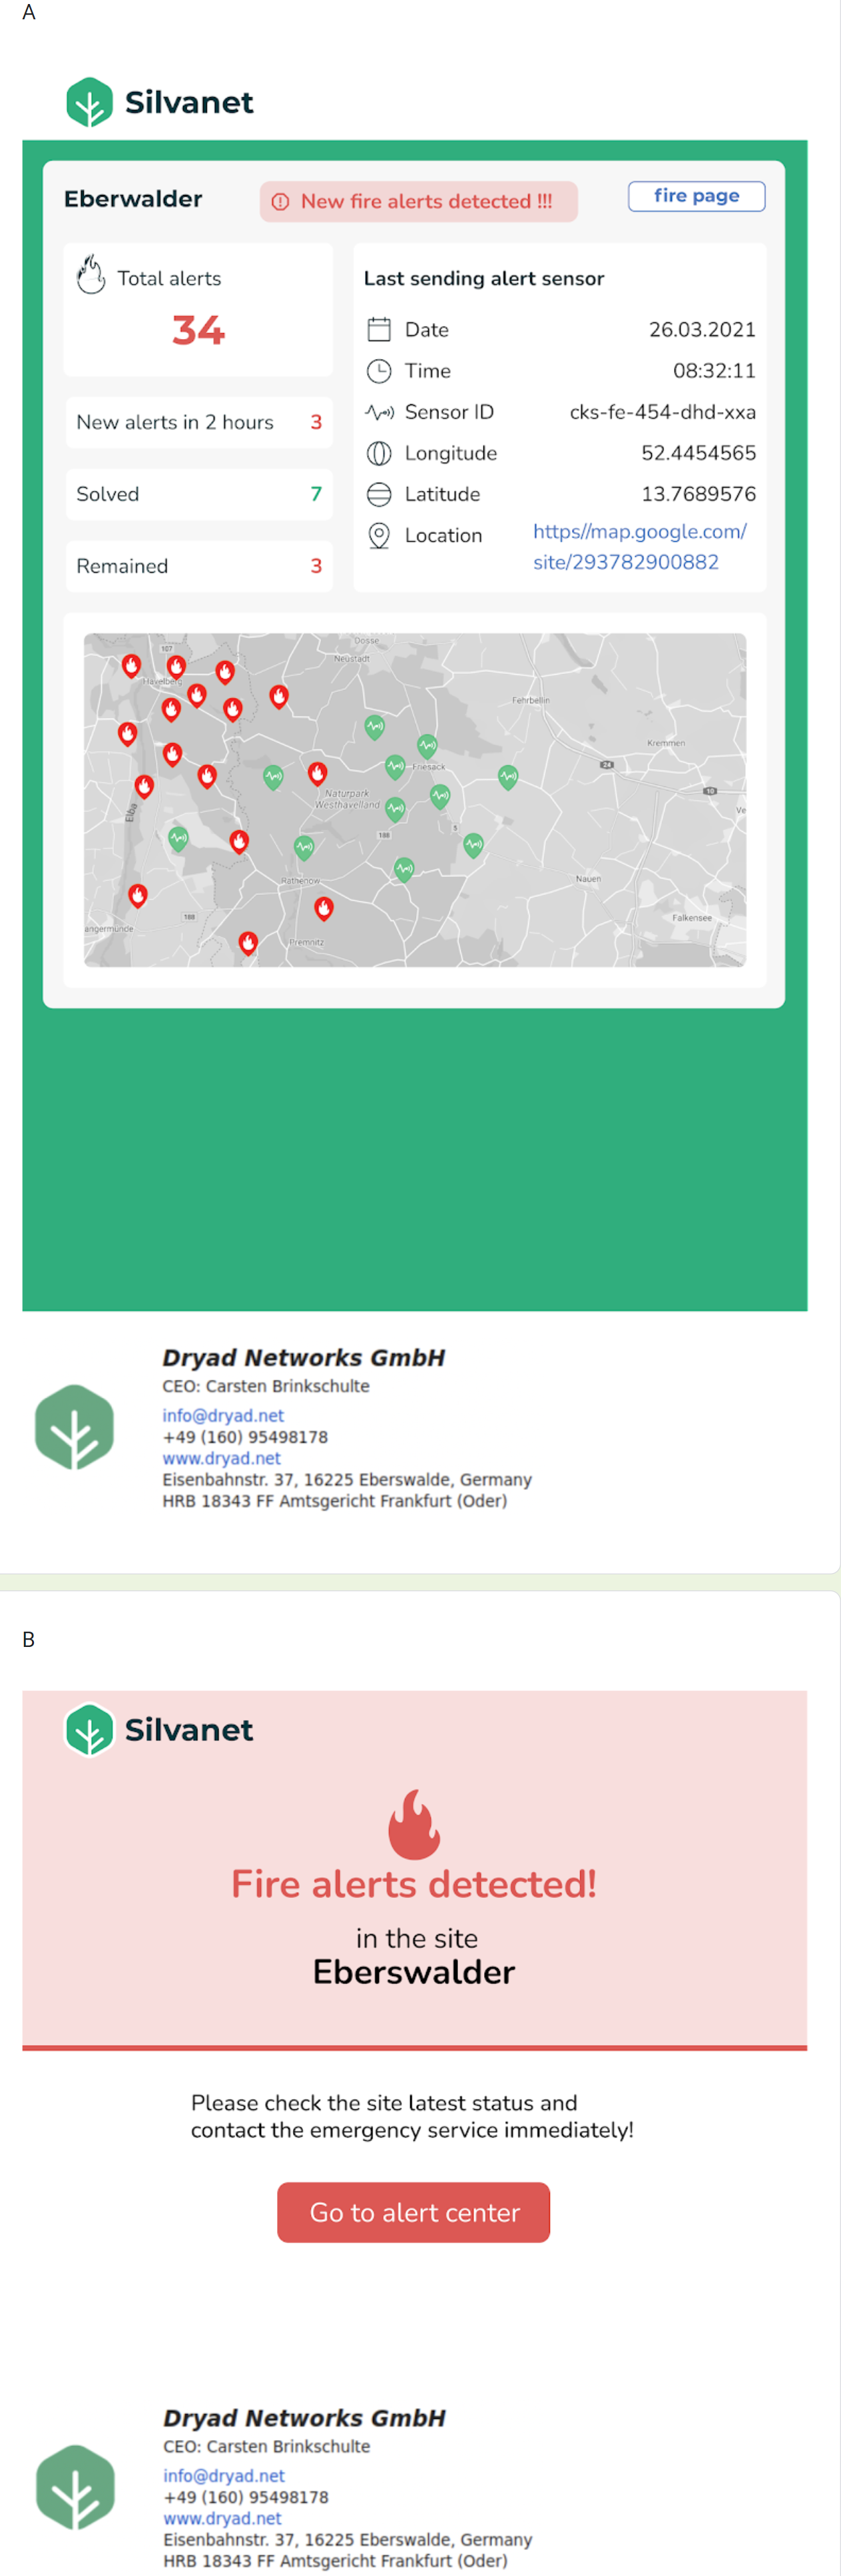
\includegraphics[width=8cm]{survey_ab_mail}
  \caption{Vergleich zweier E-Mail-Designs, die den Nutzer über die Entdeckung eines Waldbrandes durch das Silvanet-System benachrichtigen.}
  \label{fig:survey_ab_mail}
\end{figure}

Zusammenfassend lässt sich sagen, dass diese Benutzertests die Annahme bestätigten, dass interaktive Karten schwer zu verwenden sind, dass der Benutzer sich den Daten nahe fühlen möchte und dass das Hauptfeature der Waldbranderkennung und -verwaltung in Bezug auf die Kontaktaufnahme mit den lokalen Entscheidungsträgern nutzbar ist.

